\documentclass[conference]{IEEEtran}
\IEEEoverridecommandlockouts
\usepackage{cite}
\usepackage{amsmath,amssymb}
\usepackage{graphicx}
\usepackage{booktabs}
\usepackage{xcolor}
\usepackage{array}
\usepackage[hidelinks]{hyperref}
\usepackage{microtype}
\usepackage{tikz}
\usetikzlibrary{arrows.meta,positioning,shapes.geometric,calc,fit,backgrounds}
\usepackage[strings]{underscore} % allow long monospace identifiers to break at underscores in the census table

% tighten float/text separation slightly to keep the bibliography on the final page
\setlength{\textfloatsep}{5pt plus 2pt minus 2pt}
\setlength{\dbltextfloatsep}{4pt plus 2pt minus 2pt}
\setlength{\floatsep}{5pt plus 2pt minus 2pt}

% lightweight helpers
\newcommand{\rec}{\textcolor{recblue}{\textbf{recoverable}}}
\newcommand{\non}{\textcolor{noid}{\textbf{non-identifiable}}}
\definecolor{okgreen}{HTML}{009E73}
\definecolor{recblue}{HTML}{0072B2}
\definecolor{noid}{HTML}{D55E00}
\definecolor{panelgrey}{HTML}{5B6770}
\definecolor{surfacefill}{HTML}{EAF1F7}
\definecolor{surfaceedge}{HTML}{38678F}
\definecolor{enginefill}{HTML}{E2EEE8}
\definecolor{engineedge}{HTML}{2F7D5B}
\definecolor{recfill}{HTML}{CFE3F2}
\definecolor{nonfill}{HTML}{F8DDCB}
\definecolor{gatefill}{HTML}{FBE6C9}
\definecolor{gateedge}{HTML}{E69F00} % one gate gold across TikZ + matplotlib
\definecolor{blockfill}{HTML}{F4F4F4}
\definecolor{panelblue}{HTML}{F4F8FB}
\definecolor{panelwarm}{HTML}{FAF7F4}
% NCU identifiers: 6.5pt, darker gray, hyphen-free breaks at _ and . (via \url)
\newcommand{\gid}[1]{{\fontsize{6.5}{7.8}\selectfont\color{black!55}\url{#1}}}
% positioning-table capability marks (Table tab:positioning)
\newcommand{\cm}{\checkmark}
\newcommand{\xm}{{\color{black!40}$\times$}}

% ---- shared TikZ vocabulary for the architectural / workflow figures -------
% One grammar across all diagrams: rounded 2pt corners, 0.9pt strokes, pastel
% fill + darker border per role, bold name line + gray detail line per node,
% Stealth arrows, dashed = unavailable/blocked, solid band = privilege wall.
\tikzset{
  >={Stealth[length=2.6mm,width=2.0mm]},
  surf/.style={rectangle, draw=surfaceedge, line width=0.9pt, rounded corners=2pt,
               fill=surfacefill, inner sep=3pt, align=center, font=\scriptsize},
  stack/.style={rectangle, draw=black!75, line width=0.9pt, rounded corners=2pt,
                fill=white, inner sep=3pt, align=center, font=\scriptsize},
  hw/.style={rectangle, draw=black!85, line width=1.1pt, rounded corners=2pt,
             fill=black!14, inner sep=3pt, align=center, font=\scriptsize},
  engine/.style={rectangle, draw=engineedge, line width=0.9pt, rounded corners=2pt,
                 fill=enginefill, inner sep=3pt, align=center, font=\scriptsize},
  blocked/.style={rectangle, draw=black!50, line width=0.8pt, dashed,
                  rounded corners=2pt, fill=blockfill, inner sep=3pt,
                  align=center, font=\scriptsize, text=black!60},
  rectile/.style={rectangle, draw=black, line width=0.9pt, rounded corners=2pt,
                  fill=recblue, text=white, inner sep=3pt, align=center,
                  font=\scriptsize},
  nontile/.style={rectangle, draw=black, line width=0.9pt, rounded corners=2pt,
                  fill=noid, text=white, inner sep=3pt, align=center,
                  font=\scriptsize},
  gate/.style={diamond, draw=gateedge, line width=1.0pt, fill=gatefill,
               aspect=1.55, inner sep=1.2pt, align=center, font=\scriptsize},
  quarantine/.style={rectangle, draw=panelgrey, line width=0.8pt, densely dashed,
                     rounded corners=2pt, fill=white, inner sep=3.5pt,
                     align=center, font=\scriptsize, text=panelgrey},
  panel/.style={rectangle, rounded corners=4pt, inner sep=0pt},
  flow/.style={->, line width=0.9pt, draw=black!70},
  denyline/.style={line width=0.8pt, densely dashed, draw=black!45},
  detail/.style={font=\scriptsize, text=black!55},
}
% gray detail line inside a node: same size, lighter weight via color
\newcommand{\nodedetail}[1]{{\color{black!55}#1}}

\begin{document}

\title{Seeing a GPU from the Outside:\\
Counter-Free Performance Observability for Non-Privileged GPU Tenants}

\author{}

\maketitle

\begin{abstract}
GPU performance analysis normally begins with hardware performance counters,
but those counters are unavailable to ordinary users on many rented,
multi-tenant accelerators. This paper studies the resulting observability
problem: \emph{what can a non-privileged process recover about a real GPU
execution, and what is not identifiable from the legal signals?}
We present a counter-free profiling framework that combines user-space
instruction tracing, unprivileged timing, static binary inspection, and
read-only device status. The framework is evaluated on two GPU generations
and an industrial kernel benchmark; surviving validation records substantiate
127 correctness-passed Blackwell ports and 178 completed Ampere rows, the
recovered final availability summary covers 222/235 and 225/235 problems on
the two cards, and scored cache-prediction cohorts hold mean absolute error
to $0.03$--$0.06$ against locally collected Nsight Compute reference
measurements. At the
metric level, the framework reproduces one essential traffic counter exactly
from a user-space trace (geometric-mean relative error
$2.7\times10^{-12}$ over 39 held-out configurations, with no fitted
parameters), recovers a second with a statistically verified error bar at
error $157\times$ below the strongest analytic baseline, and estimates the
L2 hit ratio of memory-streaming kernels to a median error of $0.04$. The
same evaluation establishes a structural boundary: for tensor-core kernels
and other kernels that reuse data after staging it on chip, the L2 hit ratio
is not identifiable from the current legal signals because the relevant reuse
occurs in scratchpad or registers rather than in the global-address stream.
The result is an identifiability map for non-privileged GPU profiling:
accepted estimates where the legal signals determine the metric, and
testable explanations where they do not.
\end{abstract}

\begin{IEEEkeywords}
GPU performance measurement, non-root profiling, hardware performance counters,
cache modeling, identifiability, uncertainty quantification.
\end{IEEEkeywords}

\section{Introduction}

Graphics processors run a growing share of the world's computation, and when a
GPU program is too slow the first step is to \emph{measure} it. The standard
way to do this is to read the chip's built-in \emph{performance counters}:
small registers that tally cache hits, stalled cycles, and memory transactions
as the program runs.

A quiet shift has made this harder than it sounds. The large GPUs that most need
careful measurement increasingly live in rented, multi-tenant clouds, and there
the counters are switched off for ordinary users. After a 2018 disclosure showed
that one tenant could read another's data through shared
counters~\cite{naghibijouybari2018rendered,cve_2018_6260}, the vendor began restricting counter access to
administrators by default: an unprivileged attempt fails with
\texttt{ERR\_NVGPUCTRPERM} unless the host clears a driver
restriction~\cite{nvidia_errnvgpuctrperm}, and recent toolkit releases have
removed the legacy counter interface~\cite{nvidia_cupti}. The commodity way to obtain a modern datacenter
GPU---an H200 or B200---is to rent one by the hour from a provider such as
RunPod, Vast.ai, Hyperstack, or GPUHub~\cite{cloudgpu_containers}, and these
providers hand the tenant an \emph{unprivileged container}, not the host.
Inside it the deep profilers go dark---\textbf{Nsight Compute} and every
counter-bearing \textbf{CUPTI} interface fail with a permission
error~\cite{nvidia_nsightcompute,nvidia_cupti}---and even the privileged
controls that steady a measurement (locked clocks, persistence mode) are
denied.

The community's usual response is to \emph{substitute} for the counters, and
each substitute sidesteps the question a cloud user actually faces:
cycle-level simulators rebuild the chip in software but need proprietary
configurations and run orders of magnitude slower than the
hardware~\cite{bakhoda2009gpgpusim,khairy2020accelsim,villa2021nvarchsim};
analytical and learned predictors are fast but are calibrated against
counters---when the counters disappear, so does their ground
truth~\cite{hong2009analytical,lee2022gcom}; roofline and
speed-of-light analyses need no counters but report a best-case ceiling, not
what a particular run achieved~\cite{williams2009roofline}. None of them tells
a non-privileged user what is \emph{knowable} about a real execution on real
silicon, from the outside.

\smallskip
\noindent\textbf{Our question.} \emph{Given only the signals a non-privileged
process may legally observe, how much of a GPU program's internal behavior can
be recovered, and how much is absent from those signals?}

\smallskip
\noindent\textbf{What we built.} We build the profiler that question implies:
one that reads only the signals an unprivileged process may legally observe
and tells the tenant, with evidence, what those signals do and do not
determine. The framework targets a published 235-problem kernel benchmark
using native CUDA~C++/CUTLASS profiling targets, and the surviving
validation records show 127 correctness-passed Blackwell ports and 178 completed Ampere
rows (\S\ref{sec:framework}). Its accepted outputs carry guarantees that, to
our knowledge, no existing counter substitute provides (Table~\ref{tab:positioning}):
one essential counter reproduced to machine precision (the
L1$\rightarrow$L2 read-sector count: geometric-mean relative error
$2.7\times10^{-12}$ over 39 held-out configurations, with no fitted
parameters); a second carrying a distribution-free error bar whose coverage
is statistically verified, at error $157\times$ below the strongest analytic
baseline (the write-sector count); and, where the current legal signals lack
the required information, a testable explanation rather than a guess.

\smallskip
\noindent\textbf{What makes those guarantees possible: a map, not a guess.}
Rather than claim to predict
everything, we build an \emph{identifiability map}: for each quantity, a verdict
on whether it is even \emph{in principle} determinable from what we observe---the
question of structural
identifiability~\cite{villaverde2016structural}, asked
before any estimation. Exactness and verified coverage are claimable
precisely because the acceptance rule is allowed to say \emph{no}: each
metric receives one of two verdicts:
\begin{itemize}
\item \rec: a principled estimate exists; we \emph{accept} it only if it
beats the strongest baseline (and \emph{decline} it otherwise). Where the
calibration permits, we attach
an error bar whose coverage we verify.
\item \non: no principled estimate is possible. Instead of a number we issue a
\emph{testable explanation}: the physical reason the quantity is invisible, plus the
new unprivileged observation that would overturn the verdict.
\end{itemize}
The most coveted cache
metric---the large shared cache's hit ratio---is recoverable with low error for
simple memory-streaming kernels, yet \emph{not identifiable from the current legal signals} for the
matrix-multiply and register-spill kernels that dominate modern AI, because
those kernels reuse their data \emph{on-chip}, in scratchpad and
thread-private storage a user-space global-address trace never sees. We show this per workload
family, name the mechanism in each case, and corroborate every recovered number
with an independently written checker.

\smallskip
\noindent\textbf{Contributions.} The paper makes three contributions under
one rule throughout: never use a privileged interface at deployment time.

\begin{enumerate}
\item \textbf{A counter-free measurement method and an identifiability map}
(\S\ref{sec:method}--\ref{sec:map}). We recover GPU performance metrics from
user-space instrumentation alone, label each recoverable or non-identifiable,
attach a coverage-checked error bar where the calibration allows, and issue
testable explanations for the rest---to our knowledge the first
identifiability-style account of \emph{what this non-privileged observation
set can and cannot determine} about a GPU run. Every verdict is tied to the
signals actually observed, so the map can be revisited when new legal signals
are added.

\item \textbf{A cross-generation validation of the recoverable and
non-identifiable regions}
(\S\ref{sec:map}). We validate accepted estimates against local Nsight
Compute reference measurements, verify interval coverage on held-out data, and show that
the L2-hit-ratio boundary follows workload mechanism rather than average
suite behavior: streaming kernels are recoverable, while tensor-core,
normalization, intermediate-buffer, and spill families erase the needed reuse
from the global-address stream.

\item \textbf{A counter-free profiling framework at benchmark scale}
(\S\ref{sec:framework}). We realize the same method as a toolkit of five
permission-free measurement channels that \emph{records} which channels work
on each host rather than silently pretending a kernel was profiled, hand-port
benchmark kernels into native CUDA~C++/CUTLASS so the local reference
measurements profile the kernel itself rather than a Python launch layer, and report the
benchmark coverage supported by surviving validation records. Recovered final
availability status is reported separately from directly verified statistical
claims.
\end{enumerate}

\noindent Our primary measurements come from a current-generation laptop GPU (RTX
5060, Blackwell). A cross-architecture study on an older desktop GPU (RTX 3090 Ti,
Ampere) is complete: the write-traffic recovery carries over
(the read count, exactly recovered on Blackwell, is declined on Ampere), and
the large-cache identifiability boundary is confirmed on Ampere as
well---recoverable for streaming kernels, not identifiable from the current
legal signals once data is reused on-chip. Throughout, we fix accuracy targets and the workload partition
before scoring, verify every interval's coverage, reject corrections that fail
their own holdout, and report missed targets as misses rather than relax
them---a discipline we treat as a first-class contribution in a subfield where
unbacked point predictions are common practice.

\section{Background and Related Work}
\label{sec:related}

\textbf{The measurement contract.} On hosts that keep the post-CVE-2018-6260
default counter restriction in place, an ordinary process receives
\texttt{ERR\_NVGPUCTRPERM} from \textbf{Nsight Compute} and every
counter-bearing \textbf{CUPTI} profiling interface~\cite{nvidia_errnvgpuctrperm,nvidia_nsightcompute,nvidia_cupti};
clock locking is also administrative. The documented remedies are root,
a host-side driver option, or an administrative container capability, all
outside the rented-container tenant's control. The surviving substrate is
thin but real: \textbf{NVBit}/SASS instrumentation~\cite{villa2019nvbit,stephenson2015sassi},
\textbf{CUPTI Activity} and CUDA events~\cite{nvidia_cupti_activity},
static binary inspection~\cite{nvidia_cudabinutils}, \textbf{Nsight Systems}
and compute-sanitizer for availability/correctness evidence, and read-only
\textbf{NVML} covariates~\cite{nvidia_nvml}; \textbf{Nsight Compute} is used
only offline for local reference measurements.

Prior substitutes relax at least one of those premises. Cycle-level simulators
such as GPGPU-Sim, Accel-Sim, and NVArchSim rebuild the chip and validate
against privileged counters~\cite{bakhoda2009gpgpusim,khairy2020accelsim,villa2021nvarchsim};
analytical and learned models report suite-averaged timing errors while
treating cache hit rates as inputs, not counter-free outputs~\cite{hong2009analytical,lee2022gcom,lee2025neusight};
roofline analyses bound attainable performance rather than measure a
particular run~\cite{williams2009roofline,yang2020hierarchical}. Trace-driven
cache models and reuse-distance systems do predict hit rates from addresses,
but their published accuracy is earned mainly on streaming-era suites rather
than tensor-core, \texttt{cp.async}/TMA, and attention-style kernels
~\cite{nugteren2014gpucache,kiani2018reuse,arafa2021pptgpu,arafa2020reuse}.
Our distinction is not the trace itself; it is the adjudication: each family
receives a verified estimate or a testable explanation of non-identifiability. The
supporting tools and theory are classical reuse distance~\cite{mattson1970},
conformal prediction~\cite{vovk2005alrw}, structural
identifiability~\cite{villaverde2016structural}, and the microbenchmarking
lineage that fixes cache geometry without counters~\cite{wong2010demystifying,mei2017dissecting,jia2018volta,jarmusch2025blackwell}.

\begin{table}[t]
\centering
\caption{\textbf{What each counter substitute hands a non-privileged
tenant.} ``Measures the run'': reports on an actual execution of the
tenant's own kernel on real silicon, without privilege. ``Verified error
bars'': per-estimate uncertainty whose coverage is checked, rather than a
suite-averaged accuracy. ``Per-family verdicts'': accuracy judged per
workload family instead of averaged across a suite. ``Non-identifiability
explanations'': testable reasons why a metric cannot be determined from the
observed signals at all. A cross means outside the method's stated contract, not a
claim that the method is unhelpful for its own purpose.}
\label{tab:positioning}
\setlength{\tabcolsep}{2pt}
\renewcommand{\arraystretch}{1.1}
\scriptsize
\begin{tabular}{@{}l@{\hspace{4pt}}cccc@{}}
\toprule
& \textbf{\shortstack[c]{measures\\the run}}
& \textbf{\shortstack[c]{verified\\error bars}}
& \textbf{\shortstack[c]{per-family\\verdicts}}
& \textbf{\shortstack[c]{non-id.\\explanations}}\\
\midrule
Cycle-level simulation~\cite{bakhoda2009gpgpusim,khairy2020accelsim} & \xm & \xm & \xm & \xm\\
Analytical/learned models~\cite{hong2009analytical,lee2022gcom,lee2025neusight} & \xm & \xm & \xm & \xm\\
Roofline / speed-of-light~\cite{williams2009roofline} & \xm & \xm & \xm & \xm\\
Trace-driven cache models~\cite{arafa2021pptgpu,arafa2020reuse} & \cm & \xm & \xm & \xm\\
Assembly-level probes~\cite{huang2025neutrino} & \cm & \multicolumn{3}{c}{{\color{black!55}no cache or counter metrics}}\\
\textbf{This work} & \cm & \cm & \cm & \cm\\
\bottomrule
\end{tabular}
\end{table}

\noindent In short (Table~\ref{tab:positioning}), our position relative to all of the above is: (i)~we take the
non-privileged constraint as a \emph{premise}, not an inconvenience; (ii)~we ask
the identifiability question \emph{before} the estimation question; and (iii)~we
report every answer either with a verified error bar or with a testable
explanation of the missing signal.

\section{Counter-Free Observation}
\label{sec:method}

The pipeline is simple: read only the legal signals, recover what is
recoverable, and explain the rest.

\begin{figure*}[t]
\centering
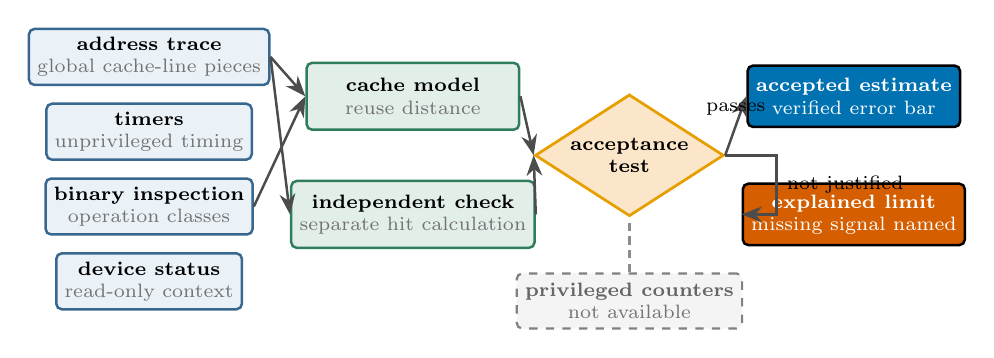
\begin{tikzpicture}[x=1cm,y=1cm]
\node[surf, minimum width=2.2cm, minimum height=0.70cm] (trace) at (0,1.25)
  {\textbf{address trace}\\\nodedetail{global cache-line pieces}};
\node[surf, minimum width=2.2cm, minimum height=0.70cm] (time) at (0,0.30)
  {\textbf{timers}\\\nodedetail{unprivileged timing}};
\node[surf, minimum width=2.2cm, minimum height=0.70cm] (static) at (0,-0.65)
  {\textbf{binary inspection}\\\nodedetail{operation classes}};
\node[surf, minimum width=2.2cm, minimum height=0.70cm] (nvml) at (0,-1.60)
  {\textbf{device status}\\\nodedetail{read-only context}};

\node[engine, minimum width=2.7cm, minimum height=0.85cm] (replay) at (3.35,0.75)
  {\textbf{cache model}\\\nodedetail{reuse distance}};
\node[engine, minimum width=2.7cm, minimum height=0.85cm] (checker) at (3.35,-0.75)
  {\textbf{independent check}\\\nodedetail{separate hit calculation}};
\node[gate, minimum width=1.55cm, minimum height=1.0cm] (gate) at (6.10,0)
  {\textbf{acceptance}\\\textbf{test}};
\node[rectile, minimum width=2.45cm, minimum height=0.78cm] (accept) at (8.95,0.75)
  {\textbf{accepted estimate}\\\nodedetail{\color{white}verified error bar}};
\node[nontile, minimum width=2.45cm, minimum height=0.78cm] (cert) at (8.95,-0.75)
  {\textbf{explained limit}\\\nodedetail{\color{white}missing signal named}};
\node[blocked, minimum width=2.2cm, minimum height=0.70cm] (priv) at (6.10,-1.85)
  {\textbf{privileged counters}\\\nodedetail{not available}};

\draw[flow] (trace.east) -- (replay.west);
\draw[flow] (static.east) -- (replay.west);
\draw[flow] (trace.east) -- (checker.west);
\draw[flow] (replay.east) -- (gate.west);
\draw[flow] (checker.east) -- (gate.west);
\draw[flow] (gate.east) -- node[above, font=\scriptsize] {passes} (accept.west);
\draw[flow] (gate.east) -- ++(0.65,0) |- node[pos=0.25, right, font=\scriptsize] {not justified} (cert.west);
\draw[denyline] (priv.north) -- (gate.south);
\end{tikzpicture}
\caption{\textbf{Counter-free profiling workflow.} The deployed tool consumes
only user-available signals. Estimates are reported only after the fixed
acceptance test verifies error and coverage; otherwise the output is a
declined estimate or a testable explanation that names the missing observation.}
\label{fig:workflow}
\end{figure*}

\subsection{The signals we are allowed to see}
\label{sec:signals}
The study consumes four classes of signal, all available to an ordinary
user; the exact capture rules---what each signal records, and what it
provably does not---are fixed before scoring.
\begin{itemize}
\item An \emph{address trace}: \textbf{NVBit}~\cite{villa2019nvbit} binary
instrumentation records, for every executed global load and store, the
addresses touched by all 32 lanes of a warp, coalesced into the 32-byte
cache-line pieces the memory system actually moves. Asynchronous staging copies
(\texttt{cp.async}) contribute their global \emph{source} addresses; their
on-chip destinations---and all bulk-tensor (TMA) transfer addresses---are
not resolved. That one boundary, as we will see, decides the central result.
\item Two \emph{unprivileged timers}---the \textbf{CUPTI Activity
API}~\cite{nvidia_cupti_activity} and \textbf{CUDA events}---reconciled
against each other for every kernel; a disagreement invalidates the measurement.
\item \emph{Static inspection} of the compiled binary~\cite{nvidia_cudabinutils}:
which memory operations are even allowed to use the cache, the register and
spill footprint, the instruction mix---offline, without running anything.
\item \emph{Read-only status readings} from \textbf{NVML}~\cite{nvidia_nvml}:
clocks, temperature, power---recorded as context, never as a model input.
\end{itemize}
The constraint is enforced mechanically, not by good intentions: the implementation
rejects, by name, any candidate model feature drawn from a hardware-counter
family, and blocklists every clock-changing option, so no privileged quantity
can leak into a deployed estimate.

\subsection{Recovering cache behavior from an address list}
\label{sec:cachemodel}
The richest counter-free signal is the list of memory addresses, and the idea
behind the recovery is sixty years old and easy to state: a cache access hits
when the data it wants was used \emph{recently enough}---formally, when its
\emph{reuse distance}, the number of distinct items touched since the last
use, fits within the cache~\cite{mattson1970}. So we run the recorded addresses through a small
software model of each card's cache hierarchy, at the same 32-byte sector
granularity the hardware accounts in, and read the hit ratio off the model.
Two safeguards keep this honest. First, every replay design choice was fixed
by a model-selection step \emph{before} scoring, and the only
correction permitted downstream is a one-dimensional calibration curve; a
classical fully associative reuse-distance
model~\cite{nugteren2014gpucache} serves as the strongest analytic baseline
the replay must beat. Second, a second, independently written reuse-distance
calculation, sharing none of the replay's machinery, re-derives every hit
ratio; the two agree on all 29 cross-checked kernel configurations. The
model is deliberately narrow---no notion of time, scheduling, or pipeline
state---and emits an estimate, never ground truth. The decisive failure case
is equally simple: when a kernel fetches a tile once and then reuses it in
scratchpad or registers, the global-address stream contains only the cold
fetches. No replay can recover reuse that never reappears in the observed
stream.

\subsection{Error bars when available, explanations when not}
\label{sec:gates}
A bare estimate is not enough, so every number the pipeline emits passes a
\emph{fixed acceptance test} that was written down before scoring. An estimate is
\emph{accepted} only if it beats the strongest baseline, and its error bar
(a distribution-free conformal interval~\cite{vovk2005alrw}) is reported only
after its claimed coverage is verified on held-out data by a statistical
test; when either check fails, we decline---a declined estimate is reported
as declined, never quietly relaxed into a pass. For a quantity we judge
non-identifiable we issue no number at all but a \emph{testable explanation}: the
physical on-chip mechanism that erases the quantity from the observable
signals, plus the specific new non-privileged observation that would overturn
the verdict. These explanations are stored before scoring, so a verdict cannot
be quietly narrowed after the fact. The result is a precise target for future
measurements, not an excuse.

\section{The Identifiability Map}
\label{sec:map}

We apply the method to the eleven essential profiler metrics a performance
engineer actually reads---the lines on a profiler's summary page: the cache
hit rates, the traffic between cache levels, main-memory traffic and
bandwidth, cycles, occupancy, instruction throughput.
The verdict on the essential set: three metrics are
recoverable and eight are non-identifiable, and recoverability lives only at
the boundary between the small on-chip cache and the interconnect, while
everything global, temporal, or throughput-related is outside the current
legal signals (Table~\ref{tab:metricmap}). The two tiers are
separated by \emph{method}, not by subject. Out of scope, deliberately:
quantities a user-space trace reproduces for free (recovering an easy count
is not a research question); near-duplicate variants of the essential
metrics, adjudicated in the supporting files rather than presented here;
and wall-clock kernel time, a property of the host's frequency governor
rather than of the kernel once clocks cannot be locked.

\begin{table*}[t]
\centering
\caption{\textbf{Identifiability map for the eleven essential summary
metrics under the current legal signals.} ``Accepted'' means the metric
passes the fixed accuracy test; ``declined'' means a principled estimator
exists but does not pass; ``not identifiable'' means the current
non-privileged signals lack the information needed for a reliable point
estimate.}
\label{tab:metricmap}
\setlength{\tabcolsep}{3pt}
\renewcommand{\arraystretch}{0.96}
\scriptsize
\begin{tabular}{@{}p{3.0cm}p{2.3cm}>{\raggedright\arraybackslash}p{11.0cm}@{}}
\toprule
\textbf{Metric} & \textbf{Verdict} & \textbf{Evidence or limitation under the current legal signals} \\
\midrule
L1$\rightarrow$L2 read sectors & \textcolor{recblue}{accepted} on Blackwell; declined on Ampere &
Exact on RTX 5060 (GMRE $2.7{\times}10^{-12}$, $n{=}39$, no fit);
Ampere misses the 90th-percentile error target on two diagnosed model effects.\\
L1$\rightarrow$L2 write sectors & \textcolor{recblue}{accepted} &
Accepted on both cards; Blackwell GMRE $5.1{\times}10^{-7}$ with
verified 90/95\% coverage (35/39, 36/39).\\
L1 sector hit rate & recoverable, declined &
Point estimator exists, but Blackwell interval hits a width floor and
Ampere bypass-class kernels dominate error.\\
L2 sector hit rate & not identifiable, family-selective &
Streaming family is below the acceptance threshold (median error $0.04$);
staged-reuse families are not identifiable from the current legal signals because reuse occurs in
scratchpad/registers, not in the global trace (Table~\ref{tab:l2family}).\\
DRAM read sectors & not identifiable &
Memory-controller coalescing/compression and unobserved partition behavior
change chip-global traffic after the trace; the missing signal is a non-counter
memory-controller transaction/residency observation.\\
DRAM write sectors & not identifiable &
Write combining and compression reshape stores below the observable trace;
the missing signal is non-privileged visibility into write-combine/compression
outcomes.\\
DRAM bandwidth & not identifiable &
Depends on hidden traffic plus non-lockable memory clocks; the missing signal is a
legal byte-transaction stream with clock-stable timing.\\
Elapsed cycles & not identifiable &
Cycle denominator is scheduler- and clock-dependent under denied clock
control; timing evidence is interval-only (\S\ref{sec:discussion}).\\
Achieved occupancy & not identifiable &
Scheduler residency is not determined by static limits or address trace;
the missing signal is a legal warp-residency/admission signal.\\
Achieved IPC & not identifiable &
Instruction totals can be counted, but the cycle denominator is
non-identifiable; the same missing cycle observation applies.\\
Memory throughput & not identifiable &
Mixes hidden DRAM traffic, stalls, and unlocked clocks; reliable recovery requires
legal byte transactions plus stable timing.\\
\bottomrule
\end{tabular}
\end{table*}

\subsection{The recoverable tier: exactness, and a verified error bar}
Three essential metrics are recoverable; two we accept and one we
deliberately decline. The two accepted metrics are data-movement
counts---the read and write traffic on the interconnect between the small
and large caches. The \emph{read} count is reproduced \emph{exactly}, to
machine precision, over 39 held-out kernel configurations and with no
fitted parameters; the address trace alone does not yield this interconnect count
directly, so the exact reproduction is a genuine recovery, not a
bookkeeping identity. The \emph{write} count is recovered by a calibrated
estimate whose error is $157\times$ below the strongest analytic baseline
and whose error bar's claimed coverage is verified on held-out data.

The third metric shows the acceptance test doing its job. The first-level cache hit
rate has a reasonable point estimate, but its verified error bar comes out
too wide to be useful---an exactly recovered traffic \emph{count} does not
pin a hit \emph{rate}---so we decline it rather than ship a number we
cannot stand behind. We could have reported all three and claimed a cleaner
score; the test is allowed to say no, and that refusal is precisely why the
accepted claims are credible.

On the second GPU generation (Ampere) the same test adjudicates metric by
metric, and the \emph{structure} carries over while one outcome flips: the
write count clears its threshold on both cards; the read count---exact on
Blackwell---misses its error budget on Ampere for two diagnosed causes
tied to persisting-window and fetch-granularity effects; and the hit-rate candidate stays
declined on both. The per-card validation numbers are summarized in
Table~\ref{tab:microbench}.


\subsection{The non-identifiable tier, and the boundary of the knowable}
\begin{table}[t]
\centering
\caption{\textbf{Central result, normalized to its fixed acceptance threshold.} Error
in the recovered L2 hit ratio per kernel family on the RTX 5060: the median
$|$predicted $-$ true$|$ (hit-ratio fraction), the same error as a multiple
of the fixed acceptance threshold ($0.055$), and the verdict with the
hidden mechanism. The pass/limit split follows the
mechanism, not error magnitude; an independently written checker
agrees on all 29 scoreable cells, and the RTX 3090 Ti confirms the same
boundary structurally (Section~\ref{sec:map}).}
\label{tab:l2family}
\setlength{\tabcolsep}{3pt}
\renewcommand{\arraystretch}{1.15}
\scriptsize
\begin{tabular}{@{}l@{\hspace{5pt}}ccc>{\raggedright\arraybackslash}p{3.0cm}@{}}
\toprule
\textbf{Kernel family} & $n$ & \textbf{median error} &
$\times$\textbf{threshold} & \textbf{Verdict: hidden mechanism} \\
\midrule
memory streaming & 6 & $0.04$ & $0.8\times$ &
\textcolor{recblue}{\textbf{recoverable}}: reuse re-traverses global
memory---below the threshold \\
\addlinespace[1.5pt]
reduction / normalize & 7 & $0.32$ & $5.9\times$ &
\textbf{above threshold} $\Rightarrow$ \textcolor{noid}{\textbf{not identifiable}}:
cross-group partial-sum
reuse unseen \\
\addlinespace[1.5pt]
intermediate buffers & 7 & $0.13$ & $2.4\times$ &
\textcolor{noid}{\textbf{not identifiable}}: cache-resident
staging buffers unseen \\
\addlinespace[1.5pt]
matrix multiply & 9 & $0.92$ & $16.7\times$ &
\textcolor{noid}{\textbf{not identifiable}}: operand tiles
staged on-chip (\texttt{cp.async}) \\
\addlinespace[1.5pt]
register spill & 0 & --- & --- &
\textcolor{noid}{\textbf{not identifiable}}: no observed
case to score; reuse is thread-private \\
\bottomrule
\end{tabular}
\end{table}

Eight essential metrics are non-identifiable---the large cache's hit
ratio, main-memory read and write traffic, main-memory bandwidth, elapsed
cycles, occupancy, instruction throughput (IPC), and memory
throughput---and every one carries a
testable explanation. The most instructive case is the large-cache hit
ratio (Table~\ref{tab:l2family}).

Evaluated per \emph{workload family}, the recovered L2 hit ratio shows a
sharp boundary. For memory-streaming kernels---whose data flows straight
through the global memory the address trace can see---the estimate has low error
(a median of $0.04$, below the accuracy threshold; $n{=}6$---too few cells to
verify an error bar, so a point verdict). For the kernels that dominate modern
AI it collapses: normalization and reduction kernels reach $0.32$ error,
intermediate-buffer kernels $0.13$, matrix-multiply (tensor-core) kernels
$0.92$---a near-total failure of the current legal signals---and register-spill
kernels admit \emph{no} estimate at all, because there is no observed case to
score.

The reason is uniform and physical. A user-space address trace records \emph{global}
memory addresses, but these kernels achieve their reuse \emph{on-chip}:
matrix-multiply stages operand tiles through scratchpad with asynchronous copies
(\texttt{cp.async}/\texttt{LDGSTS}); normalization reuses partial sums
\emph{across} cooperating thread groups; intermediate-buffer kernels keep
producer results cache-resident without re-traversing the global path; register spills live in
thread-private local memory, whose addresses a global-address trace does not
carry. Almost none of that on-chip residency
reaches a global-address trace, so the model under-predicts (normalization,
intermediate buffers) or floors (matrix-multiply, spill). We do not paper over this with a
fitted correction; we mark the limit per family, always relative to the
fixed observation set of \S\ref{sec:signals}. The matrix-multiply explanation is:
\emph{metric}~=~L2 hit ratio; \emph{mechanism}~=~operand tiles staged into
scratchpad by asynchronous copies whose global fetches the trace does record
but whose scratchpad destinations---and the on-chip reuse they feed---generate
no further global traffic;
\emph{needed observation}~=~a non-privileged sampler that resolves staging-copy
destinations or on-chip residency. That observation is plausible in
principle---it is exactly what staged-destination resolver and
bulk-tensor decoder components are designed to expose, and
programmable-probe frameworks already observe instruction operands in flight
under the same non-privileged constraint~\cite{huang2025neutrino}---so the
explanation is a concrete research bet, not a vague caveat. The trace
itself is faithful---it reproduces the reference access stream---so the failure
is not a bad recording but on-chip reuse the trace cannot express.

\noindent\textbf{Ampere confirms the boundary.} On the RTX 3090 Ti we reach the
same per-family verdict: the L2 hit ratio is recoverable for streaming
kernels and not identifiable from the current legal signals once data is reused on-chip. A calibrated
estimator does reach the aggregate accuracy threshold there---and we
\emph{decline} it anyway, because it fails its robustness checks: drop a
single kernel from the fit and the answer moves, which makes it an overfit,
not a measurement (GMRE $0.064$, but $0.34$ leave-one-out gap and $0.71$
leave-one-kernel-out change). What Ampere
confirms is therefore not a fitted number but the \emph{mechanism}: the
same hidden-reuse mechanism---on-chip staged reuse invisible to a global-address
trace---operates on both generations, so the identifiability boundary is
stable across hardware.


\subsection{How the verdicts were validated}
\label{sec:microbench}
The quantitative recoverable verdicts and the L2 boundary rest on a fixed
microbenchmark suite spanning the five families of Table~\ref{tab:l2family}---70
admitted kernel/shape cells across the two cards, plus the traffic counts'
separate held-out trace cohorts---each cell scored against a locally produced
Nsight Compute reference measurement, in the error metrics the literature itself uses:
geometric-mean
relative error as in the analytical-model
lineage~\cite{hong2009analytical,lee2022gcom}, MAPE and Pearson correlation
as in simulator validation~\cite{bakhoda2009gpgpusim,khairy2020accelsim}
(Table~\ref{tab:microbench}). One reading from that validation is central:
\textbf{correlation flatters}. An estimator we \emph{decline} still tracks
the reference measurements at $r{=}0.94$, because counts spanning decades of magnitude
correlate almost automatically; our acceptance tests therefore act on per-cell error
and verified coverage, never on $r$. Every non-accepted cell carries a
diagnosed cause. The remaining non-cache limitations are
validated against the current legal signals: each names the hidden mechanism and
the legal observation that would be required to turn it into an estimate.

\begin{table}[t]
\centering
\caption{\textbf{Microbenchmark validation against the locally produced NCU
reference measurements.} Every cell is accepted, declined, or marked
non-identifiable; no suite average hides a failed family. GMRE $=$ geometric-mean
relative error; MAPE $=$ mean absolute percentage error; p90 $=$ 90th percentile.}
\label{tab:microbench}
\setlength{\tabcolsep}{3pt}
\renewcommand{\arraystretch}{1.0}
\scriptsize
\begin{tabular}{@{}p{1.35cm}>{\raggedright\arraybackslash}p{3.35cm}>{\raggedright\arraybackslash}p{3.35cm}@{}}
\toprule
\textbf{Metric} & \textbf{RTX 5060 (sm\_120)} & \textbf{RTX 3090 Ti (sm\_86)} \\
\midrule
L1$\rightarrow$L2 read sectors & \textbf{accepted}: exact, GMRE
$2.7{\times}10^{-12}$ ($n{=}39$) & \textbf{declined}: p90 $0.51$ vs $0.25$;
11/13 exact; MAPE 19\%, $r{=}0.94$ \\
\addlinespace[2pt]
L1$\rightarrow$L2 write sectors & \textbf{accepted}: GMRE
$5.1{\times}10^{-7}$ ($n{=}39$); 90/95\% coverage 35/39, 36/39 &
\textbf{accepted}: p90 $0.00$; 19/20 exact; MAPE 5\%, $r{>}0.999$ \\
\addlinespace[2pt]
L1 hit rate & \textbf{declined}: interval at width floor &
\textbf{declined}: GMRE $0.89$ ($n{=}30$) \\
\addlinespace[2pt]
L2 hit ratio & \textbf{not identifiable}: family median $|$err$|$
$0.04$--$0.92$ (Table~\ref{tab:l2family}); $r{=}0.38$ ($n{=}29$);
&
\textbf{structural only}: GMRE $0.064$, declined as fitted
($0.34$/$0.71$) \\
\bottomrule
\end{tabular}
\end{table}

\begin{figure*}[t]
\centering
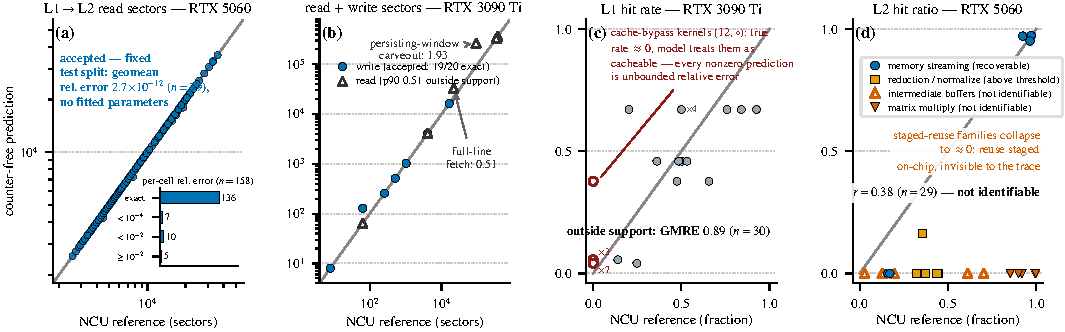
\includegraphics[width=\textwidth]{figures/fig_microbench.pdf}
\caption{\textbf{Per-cell validation against the local NCU reference measurements.}
Accepted estimates lie on the diagonal; declined estimates and
not-identifiable families show the failure modes that would be hidden by a
suite average.
Panels cover Blackwell read sectors, Ampere read/write sectors, Ampere L1
hit rate, and Blackwell L2 hit ratio by family.}
\label{fig:microbench}
\end{figure*}

\section{A Counter-Free Profiling Framework at Scale}
\label{sec:framework}

Our second contribution deploys the method where the counters are actually
locked, on SOL-ExecBench~\cite{nvidia2026solexecbench}: 235 real GPU-kernel
problems spanning L1 (94), L2 (82), Quant (33), and FIB/FlashInfer (26), where
L1/L2 are benchmark difficulty tiers rather than hardware caches. We hand-port
the measured targets from Python/PyTorch references into native CUDA~C++/CUTLASS so the
offline \textbf{Nsight Compute} reference measurements and the counter-free channels profile
the same kernel binary, not an interpreter or JIT layer.

The two local targets are an RTX 5060 laptop GPU (Blackwell, 8\,GiB) and an RTX
3090 Ti desktop GPU (Ampere, 24\,GiB). The deployed framework layers five
permission-free channels---NVBit address tracing, CUPTI Activity, Nsight
Systems timelines, static SASS inspection, and compute-sanitizer---plus
read-only NVML covariates, and records why any channel is missing: unavailable
because the host denies access, or unavailable because the kernel fails to
build, launch, or fit in memory. We report two evidence layers. The surviving
validation records substantiate a conservative directly verified floor:
\textbf{127} correctness-passed Blackwell ports and \textbf{178}
completed rows out of 201 represented Ampere rows. The
reconstructed final availability summary covers \textbf{222/235} problems on
the RTX 5060 and \textbf{225/235} on the RTX 3090 Ti, with a 226-problem
union across the two cards.\footnote{The final availability counts are
recovered from surviving summary records after loss of the detailed final
logs. They are reported as recovered completion status, not used to promote
any statistical accuracy claim.} All five channels work on the desktop host;
the laptop records Nsight Systems as unavailable because of host permissions.

The same deployment scores cache-behavior estimates against the local reference
measurements on the benchmark's own kernels. This is narrower than porting coverage:
it is the subset with both counter-free traces and a repeatable local NCU
reference measurement. On the RTX 3090 Ti, the main validation set
(34 problems across three genres) holds leave-one-out mean absolute error to
$0.033$ for L1 hit rate and $0.055$ for L2 hit ratio; the RTX 5060 held-out
cohort repeats at $0.036$/$0.038$; and the deliberately out-of-family
stress-test cases ($n{=}1$ and $n{=}2$) stay within their looser threshold.
This is calibrated prediction evidence, not a recovery verdict: the deployed
estimator is calibrated, one L2 threshold was changed in a documented update
(the original threshold would have declined it), and staged-reuse kernels
receive a family-level estimate rather than a per-kernel recovery.
Figure~\ref{fig:framework} summarizes both the availability by
benchmark genre and the calibrated cache-prediction cohorts.

\begin{figure*}[t]
\centering
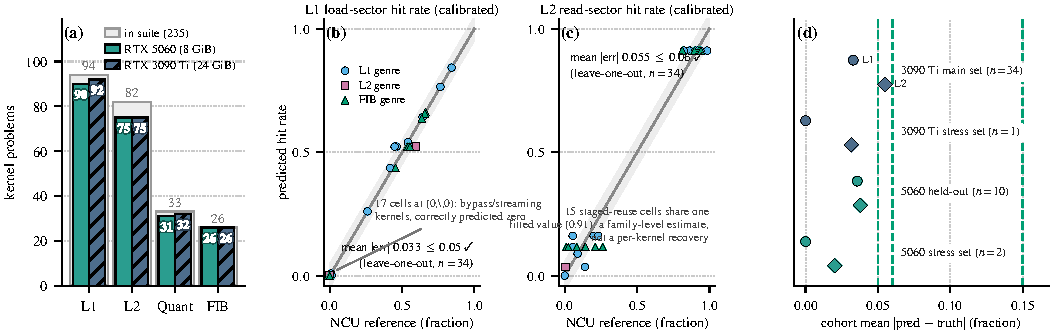
\includegraphics[width=\textwidth]{figures/fig_framework.pdf}
\caption{\textbf{Benchmark-scale framework evidence.} Panel (a) shows the
reconstructed per-genre availability on both GPUs against the 235-problem
SOL-ExecBench suite. Panels (b)--(c) compare deployed calibrated hit-rate
predictions with the local NCU reference measurements on the RTX 3090 Ti cohort. Panel
(d) reports mean-error outcomes against the thresholds on both cards; L1 points are circles
and L2 points are diamonds.}
\label{fig:framework}
\end{figure*}

\section{Recovered Completion Status and Workflow}
\label{sec:workflowstatus}

The study contains two kinds of evidence. First, the measured results in
Sections~\ref{sec:map}--\ref{sec:framework} are backed by retained measurement
records or by regenerated consistency checks that re-read those records.
Second, several late-stage completion records survived only as summary records
after the detailed final logs were lost. We include those records because they
describe the completed engineering workflow, but we do not use them to change
any accepted, declined, or not-identifiable verdict unless the underlying
measurement record also survives.

\begin{table}[!h]
\centering
\caption{\textbf{Completion workflow and surviving evidence.} ``Directly
verified'' rows are used for statistical claims in this paper. ``Recovered
status'' rows are included as completion status after loss of detailed final
logs; they are not used to promote a metric through the accuracy thresholds.}
\label{tab:status}
\setlength{\tabcolsep}{3pt}
\renewcommand{\arraystretch}{1.15}
\scriptsize
\begin{tabular}{@{}>{\raggedright\arraybackslash}p{1.65cm}>{\raggedright\arraybackslash}p{3.05cm}>{\raggedright\arraybackslash}p{3.35cm}@{}}
\toprule
\textbf{Component} & \textbf{Purpose} & \textbf{Status used in this report} \\
\midrule
Interconnect traffic recovery & Recover L1$\rightarrow$L2 read/write sector
counts from the legal address trace & \textbf{Directly verified}: Blackwell read
exact; write accepted on both GPUs; Ampere read remains declined in the
retained scored record.\\
\addlinespace[1.5pt]
L2 reuse adjudication & Decide whether L2 hit ratio is recoverable per
workload family & \textbf{Directly verified}: streaming kernels recoverable;
staged-reuse families are not identifiable from the current legal signals.\\
\addlinespace[1.5pt]
Staged-copy and TMA handling & Expose the on-chip staging destinations named
by the matrix-multiply limitation & \textbf{Recovered status}:
engineering completion is recorded, but final detailed scoring logs are
not present; verdicts therefore remain tied to the retained current-signal
evidence.\\
\addlinespace[1.5pt]
Access-class masks & Prevent bypass-class accesses from being replayed as
cacheable on Ampere & \textbf{Recovered status}: closure workflow is recorded;
the surviving Ampere L1 result remains the earlier declined result.\\
\addlinespace[1.5pt]
SOL-ExecBench availability & Port and exercise native CUDA/CUTLASS targets
across the benchmark & \textbf{Recovered status}: final availability is
222/235 on RTX 5060 and 225/235 on RTX 3090 Ti; the retained validation-record floor is
127/178 as stated in Section~\ref{sec:framework}.\\
\addlinespace[1.5pt]
Cloud-container deployment & Exercise the counter-free channels on a rented
datacenter GPU without host privileges & \textbf{Recovered status}: deployment
status is recorded as an availability audit; no counter-based reference measurement can
exist on that host without administrator access.\\
\bottomrule
\end{tabular}
\end{table}

The status split is important for interpretation. Recovered completion records
are useful for project reporting and for explaining the engineering path from
diagnosis to implementation. They are not substitutes for the detailed NCU
labels, address traces, or per-cell scoring records needed to alter the statistical
claims in Tables~\ref{tab:metricmap}--\ref{tab:microbench}. The paper therefore
keeps the strongest directly verified result where the evidence survives and
labels later recovered status as workflow evidence.

\section{Discussion and Limitations}
\label{sec:discussion}

\textbf{What the boundary means.} The limit on counter-free observability is
\emph{structural}, not statistical: the metrics we
cannot recover are those whose information never reaches the observable signals.
The map tells a practitioner which questions a non-privileged tool can answer
(interconnect traffic, the L2 hit ratio of streaming kernels) and which it cannot (on-chip
reuse), and it tells a hardware or
runtime designer which new non-privileged observable would unlock the rest.

\textbf{Evidence discipline.} We fix accuracy targets and the workload
partition before scoring, verify every error bar's coverage, cross-check every
recovered number against an independent calculation, and emit a reasoned refusal rather than a
guess. The sharpest case is on Ampere, where a
fitted L2 correction \emph{passes} the aggregate accuracy threshold and we reject it
anyway: it fails its robustness checks (\S\ref{sec:map}), and a number that
does not survive dropping a single kernel is an overfit, not a measurement. We
therefore rest the cross-architecture claim on the hidden-reuse
mechanism---identical on both generations---not on a number we could have
reported and did not. Several headline quantities do not meet their targets,
and we report them as misses.

\begin{figure}[t]
\centering
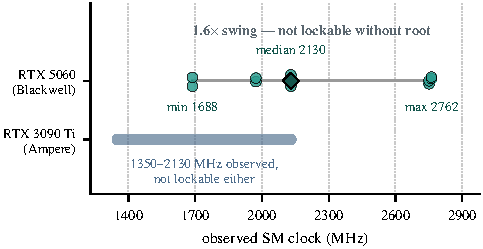
\includegraphics[width=\columnwidth]{figures/fig_timing.pdf}
\caption{\textbf{Timing is a host-governor quantity under denied clock
control.} The unprivileged timers agree with each other, but the SM
clock still moves substantially between runs, so wall-clock kernel time is
reported as an interval/limitation rather than promoted to a counter-free
architectural metric.}
\label{fig:timing}
\end{figure}

\textbf{Limitations.} Our primary measurements are from a laptop GPU (RTX 5060,
Blackwell); the cross-architecture study on a desktop GPU (RTX 3090 Ti, Ampere)
confirms the write-traffic result and the L2 boundary (the read
count flips, \S\ref{sec:map}). The cache replay models a single shared-cache partition and
does not replay every traffic class (texture-path, atomic, bulk-tensor), which are
handled with a named missing-mechanism explanation rather than scored.

Most fundamentally, the reference measurements that calibrate and check our predictions
is the privileged profiler, runnable only on local GPUs where we hold root,
while the framework is built for rented datacenter GPUs---a B200 or H200
reached through an unprivileged container---where we have neither the profiling
permission the reference measurement requires nor the clock control that makes a
measurement repeatable; the privileged reference measurement cannot be produced on that
hardware. The
counter-free channels require nothing those containers deny, so they are
built to run there unchanged; whether the locally calibrated map transfers
\emph{directly} to datacenter scale remains outside the evidence available
in this report.

\section{Conclusion}
We asked how much of a GPU's internal behavior a non-privileged observer can
recover when the hardware counters are locked away. The answer is not a
single accuracy number but a map. Some quantities are recoverable from the
legal signals: the Blackwell L1$\rightarrow$L2 read-sector count is recovered
to machine precision, the write-sector count is accepted with verified
coverage, and streaming-kernel L2 hit ratio is within its acceptance threshold. Other
quantities are structurally absent: tensor-core and staged-reuse kernels
perform the relevant reuse in scratchpad or registers, so a global-address
trace cannot identify their L2 hit ratio. The framework scales the same
evaluation discipline to SOL-ExecBench, with a retained validation-record floor of
127 correctness-passed Blackwell ports and 178 completed Ampere rows, plus a
reconstructed final availability summary of 222/235 and 225/235 problems on
the two cards. The central contribution is therefore a counter-free profiler
that reports what it can measure, refuses what it cannot justify, and turns
each refusal into a testable statement about the missing observation.

\bibliographystyle{IEEEtran}
\bibliography{refs}

\end{document}
